%\documentclass[fleqn, letterpaper]{amsart}
\documentclass[fleqn, letterpaper]{tufte-handout}
\usepackage{times}
\usepackage{amsmath}
\usepackage{amssymb}
\usepackage{graphicx}
\usepackage{booktabs}
\usepackage{multirow}
\usepackage{listings}
\usepackage{epstopdf}
\usepackage{bm}
\usepackage{natbib}
%\usepackage[left=1in]{geometry}

\newcommand{\R}{\mathcal{R}}
\newcommand{\E}{\text{E}}
\newcommand{\p}{p_{XY}}
\newcommand{\T}{^\text{T}}
\newcommand{\y}{\mathbf{y}}
\newcommand{\z}{\mathbf{z}}
\newcommand{\I}{\mathbf{I}}
\newcommand{\HH}{\mathbf{H}}
\newcommand{\A}{\mathbf{A}}
\newcommand{\GG}{\mathbf{G}}
\newcommand{\vecv}{\mathbf{v}}
\newcommand{\uu}{\mathbf{u}}
\newcommand{\cyy}{\mathbf{C}_{yy}}
\newcommand{\cuu}{\mathbf{C}_{uu}}
\newcommand{\cvv}{\mathbf{C}_{vv}}
\newcommand{\cpp}{\mathbf{C}_{\psi\psi}}
\renewcommand{\arraystretch}{1.5}
\newcommand{\KK}{\left(\begin{array}{c} \frac{{\sigma_{\y_1}}^2}{{\sigma_v}^2 + {\sigma_{\y_1}}^2}\\ \frac{\sigma_{\y_1\y_2}}{{\sigma_v}^2 + {\sigma_{\y_1}}^2} \end{array}\right)}
\newcommand{\cyylong}{\left(\begin{array}{cc} {\sigma_{y_1}}^2 & \sigma_{\y_1\y_2}\\ \sigma_{\y_1\y_2} & {\sigma_{y_2}}^2 \end{array}\right)}
\renewcommand{\vec}[1]{\mathrm{#1}}

\title{Problem Set 6 --- ENCE689E Spring 2014}
\author{David Prentiss}

\begin{document}
\maketitle

\section{1. Kalman Filter}
\subsection{(a)}
\begin{align*}
        \frac{dy}{dt} &= \phi y_t + \psi + u(t) \\
        \frac{y_{t+1}-y_t}{\Delta t} &= \phi y_t + \psi + u(t) \\
        \frac{y_{t+1}}{\Delta t} &= \phi y_t + \psi + u(t) + y_t\\
                                 &= \begin{pmatrix} \phi_1+1 & \phi_2 \\ \phi_3 &\phi_4+1\end{pmatrix} y_t + \psi + u(t)\\
        y_{t+1} &= Ay_t + b\psi + cu(t),
\end{align*}
where $A = \begin{pmatrix} \phi_1+1 & \phi_2 \\ \phi_3 &\phi_4+1\end{pmatrix}\text{ and } b = c = \Delta t
$.

\subsection{(b)}
\[z = Hy + v\]
where $ H = (1\quad 0)\T $ and $v\sim\mathcal{N}(\bar{v},\ C_{vv})$

\subsection{(c)}
\begin{align*}
\y_{t+1}^- &= \A\y_t + \GG u(t) + \GG\psi\\
&= \left(\begin{array}{c} \Delta t\, \left(\psi_1+ \uu_1\right) + \Delta t\, y_1\, \left(\phi_1 + 1\right) + \Delta t\, \phi_2 y_2\\ \Delta t\, \left(\psi_2 + \uu_2\right) + \Delta t\, y_2\, \left(\phi_4 + 1\right) + \Delta t\, \phi_3\, y_1 \end{array}\right) \\ \\
\cyy &= \A\cyy\A\T + \GG\cuu\GG\T + \GG\cpp\GG\T
\end{align*}
where $\GG = \Delta t \mathbf{I}$.
\subsection{(d)}
\begin{align*}
K &= \cyy \HH\T(\HH\cyy\HH\T+\cvv)^{-1} \\
&= \KK\\ \\
y^+ &= y^- + K(\z-\HH y^-) \\
&= y^- + \cyy \HH\T(\HH\cyy\HH\T+\cvv)^{-1}(\z-\HH y^-) \\ 
&= \left(\begin{array}{c} y_1 + \frac{{\sigma_{y_1}}^2\, \left(z - y_1\right)}{{\sigma_v}^2 + {\sigma_{y_1}}^2}\\ y_2 + \frac{\sigma_{y_1y_2}\, \left(z - y_2\right)}{{\sigma_v}^2 + {\sigma_{y_1}}^2} \end{array}\right)\\ \\
\cyy^+  &= \left(\I - K\HH\right)\cyy\\
&= \left[\left(\begin{array}{cc} 1 & 0\\ 0 & 1 \end{array}\right) - \KK (1\quad 0)\right]\cyylong\\
&= \left[\begin{array}{cc}
 {\sigma_{y_1}}^2\, \left(1 -\frac{{\sigma_{y_1}}^2}{{\sigma_\vecv}^2 + {\sigma_{y_1}}^2}\right) 
 &  \sigma_{y_1y_2}\, \left(1-\frac{{\sigma_{y_1}}^2}{{\sigma_\vecv}^2 + {\sigma_{y_1}}^2}\right)\\
  \sigma_{y_1y_2} - \frac{{\sigma_{y_1}}^2\, \sigma_{y_1y_2}}{{\sigma_\vecv}^2 + {\sigma_{y_1}}^2} 
  & {\sigma_{y_2}}^2 - \frac{{\sigma_{y_1y_2}}^2}{{\sigma_\vecv}^2 + {\sigma_{\y_1}}^2} \end{array}\right]
\end{align*}
\subsection{(e)}
\begin{align*}
\y_{t+2}^- &= \A\y_{t+1}^+ + \GG u(t+1) + \GG\psi\\ \\
\end{align*}
\subsection{(f)}
To estimate the parameter $\psi$ we could use an augmented state such as
\[\begin{pmatrix}\mathbf{y} \\ \psi\end{pmatrix}\]
and the matrix $\mathbf{A^\prime}$ would be 
\[\begin{pmatrix}\mathbf{A} & 0\\0& \mathbf{I}\end{pmatrix}\]
and
\[\begin{pmatrix}\mathbf{y} \\ \psi\end{pmatrix}_{t+1} =
\begin{pmatrix}\mathbf{A} & 0\\0& \mathbf{I}\end{pmatrix}
\begin{pmatrix}\mathbf{y} \\ \psi\end{pmatrix}_t +
\Delta t\begin{pmatrix}\mathbf{u(t)} \\ 0\end{pmatrix}
\]
\section{2. Kalman Filter}

\subsection{(a)}
\begin{align*}
\begin{pmatrix}
bf{y}_{t+1} \\
\mathbf{u}_{t+1} \\
\end{pmatrix}
&=
\begin{pmatrix}
a\mathbf{y}_t + \mathbf{u}_t \\
\rho\mathbf{u}^{(true)}_t+ \mathbf{w}_t
\end{pmatrix}
\end{align*}

\subsection{(b)}

\subsection{(c)}
{\scriptsize
        \begin{minipage}{\linewidth}
                \lstinputlisting[language=Matlab, caption={True states and forcing},
                basicstyle=\ttfamily, label=lst1]{ps6.m}
        \end{minipage}
}

See figures \ref{2ca} and \ref{2cb}.
\begin{figure}
        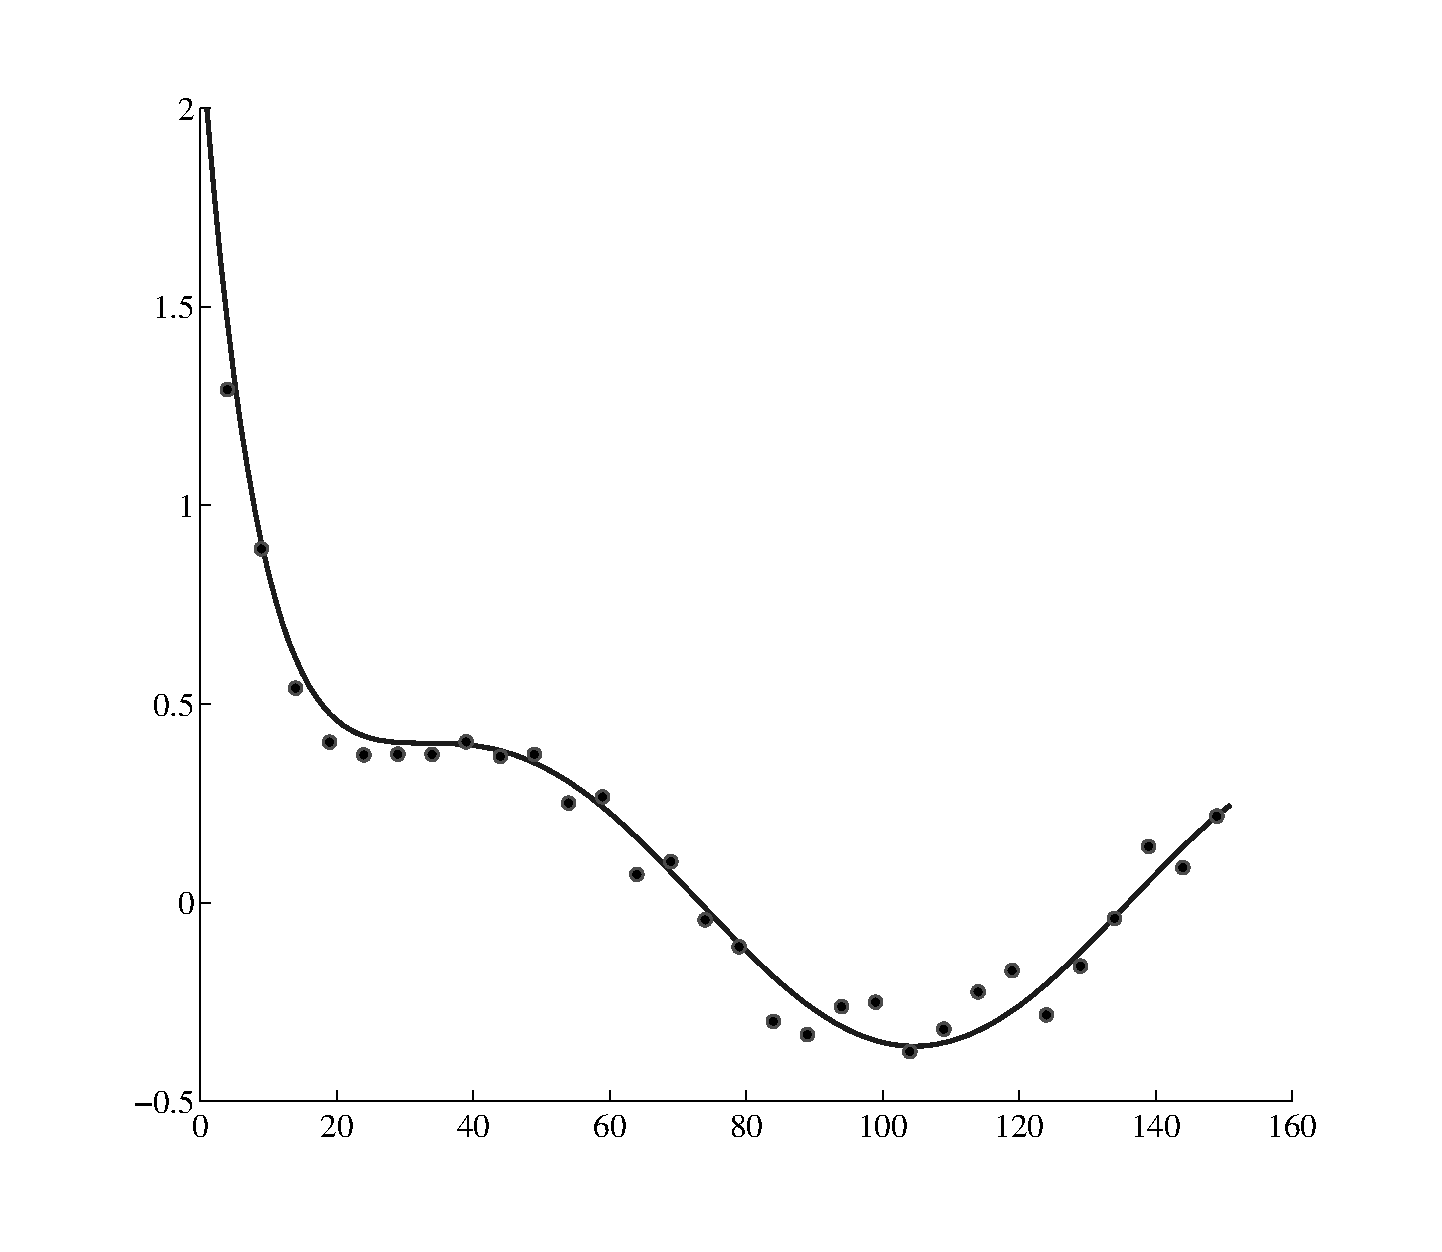
\includegraphics[width=\textwidth]{2ca}
        \caption{True, single-state system and simulated measurement error.}
        \label{2ca}
\end{figure}
\begin{figure}
        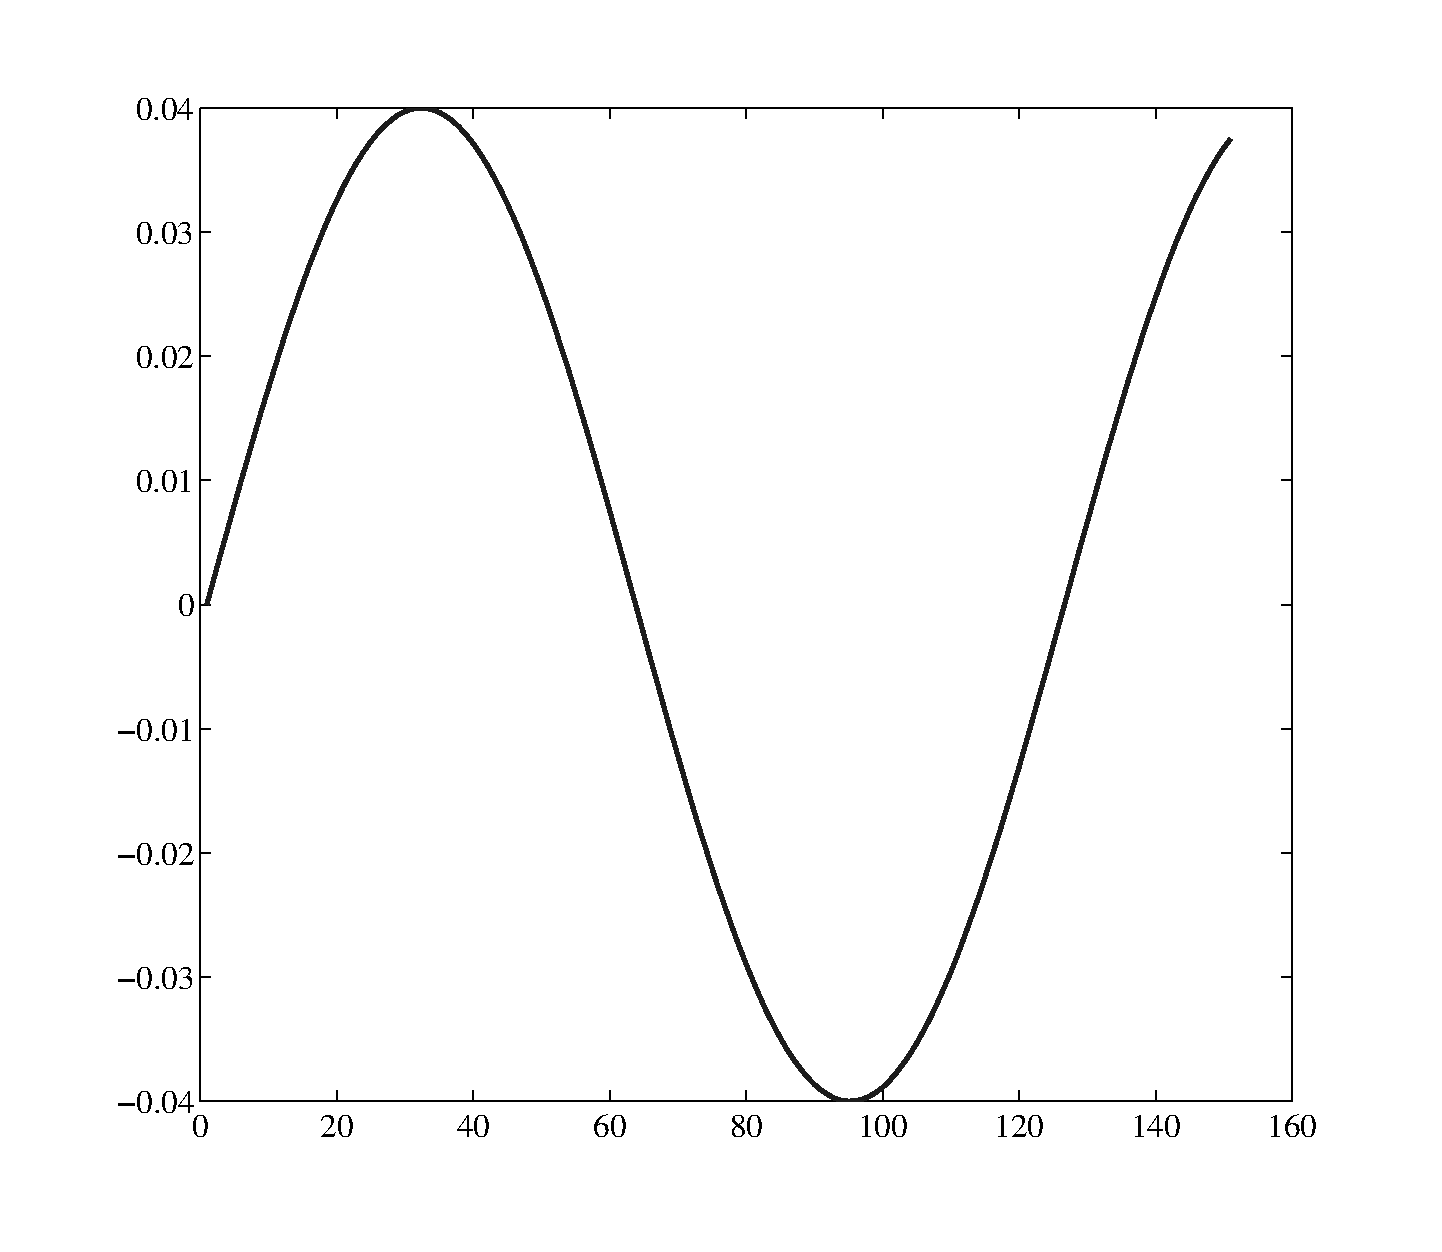
\includegraphics[width=\textwidth]{2cb}
        \caption{True model forcing}
        \label{2cb}
\end{figure}

\subsection{(d)}
From trial and error we find that the bial and RMSE improves as $\rho$ aprroaches 1. Choose 0.99.

\subsection{(e)}
From our samples of \texttt{ytrue} and \texttt{utrue} we can take the sample covariance of each and construct the variavce matrix. Since the errors are uncorrelated, only the diagonals have non-zero values.
\[
\begin{bmatrix} 0.1942 & 0 \\ 0 & 0.0008
\end{bmatrix}
\]
\subsection{(f)}
\begin{figure}
        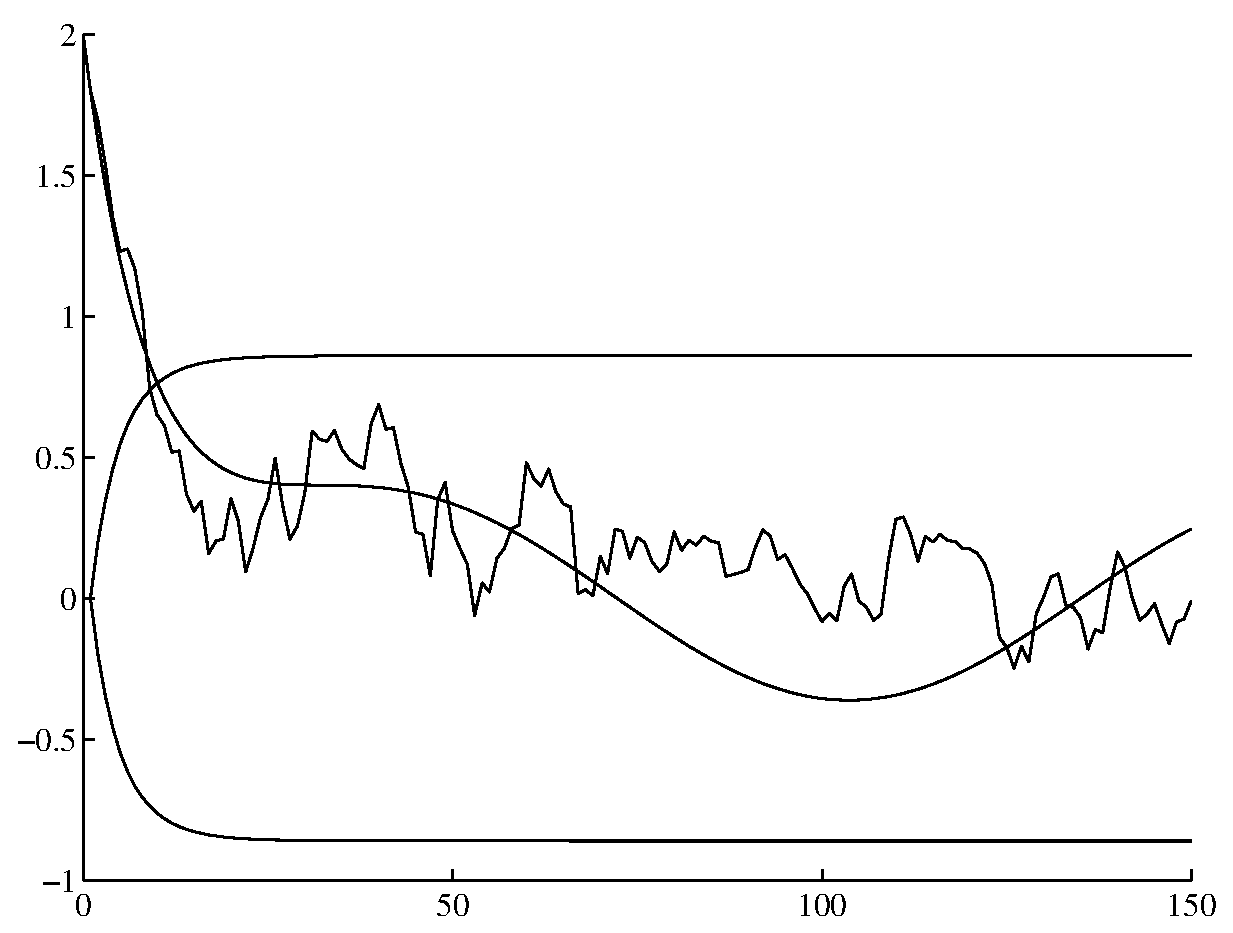
\includegraphics[width=\textwidth]{2fa}
        \caption{$\y$ and $\sigma_y$ for $\rho=0.99$}
        \label{2fa}
\end{figure}
\begin{figure}
        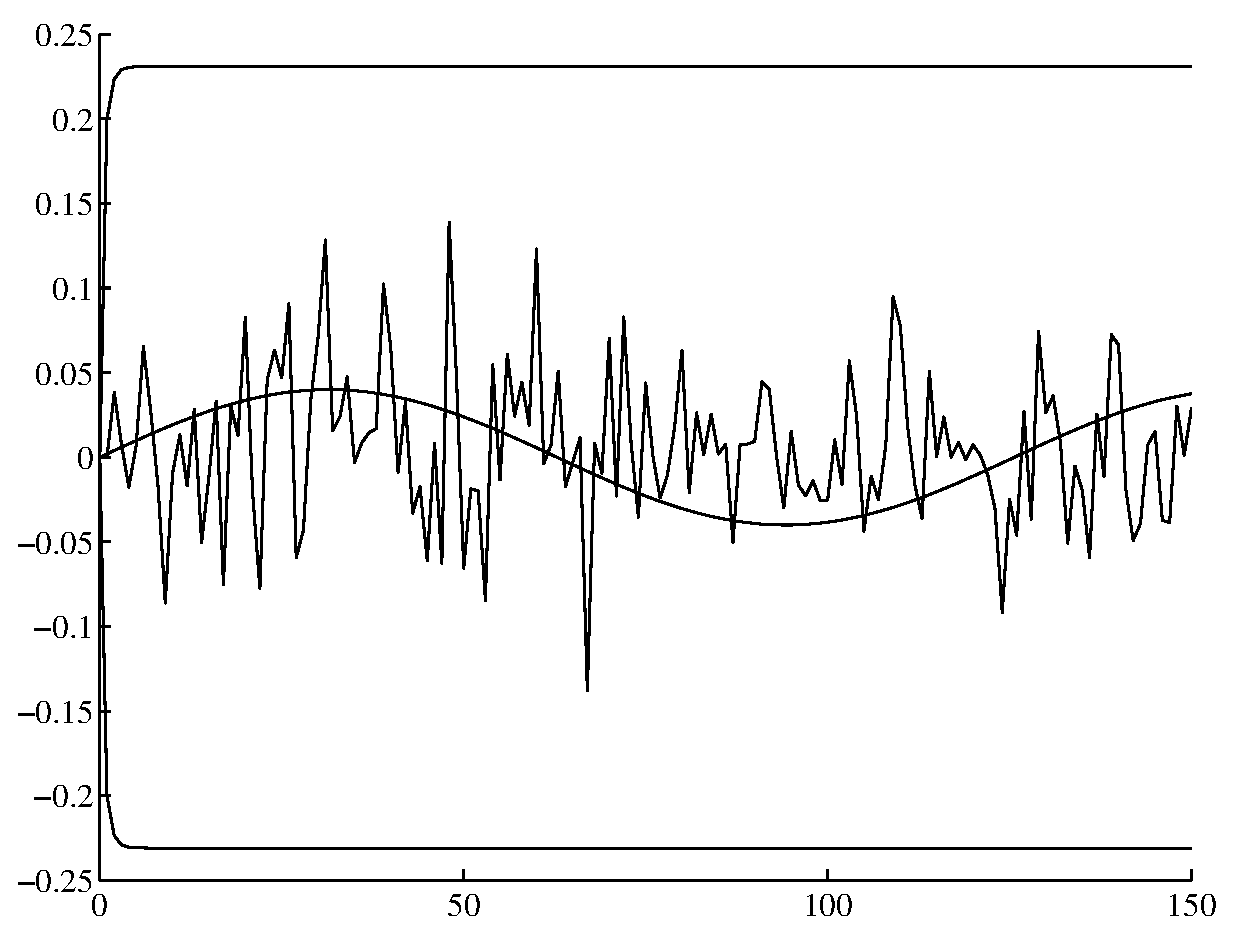
\includegraphics[width=\textwidth]{2fb}
        \caption{The forcing for $\rho=0.99$}
        \label{2fb}
\end{figure}
{\scriptsize
        \begin{minipage}{\linewidth}
                \lstinputlisting[language=Matlab, caption={Open Loop},
                basicstyle=\ttfamily, label=lst1]{ps6f.m}
        \end{minipage}
}

\begin{tabular}{ccc}
& Bias & RMSE \\
$\y$ & -0.1101 & 0.2727 \\
$u$ & -0.0028 & 0.0506
\end{tabular}

\subsection{(g)}
{\scriptsize
        \begin{minipage}{\linewidth}
                \lstinputlisting[language=Matlab, caption={Kalman filter},
                basicstyle=\ttfamily, label=lst1]{ps6g.m}
        \end{minipage}
}
\begin{tabular}{ccc}
& Bias & RMSE \\
$\y$ & 0.0026 & 0.0326 \\
$u$ & 3.9219e-04 & 0.0047
\end{tabular}

\begin{figure}
        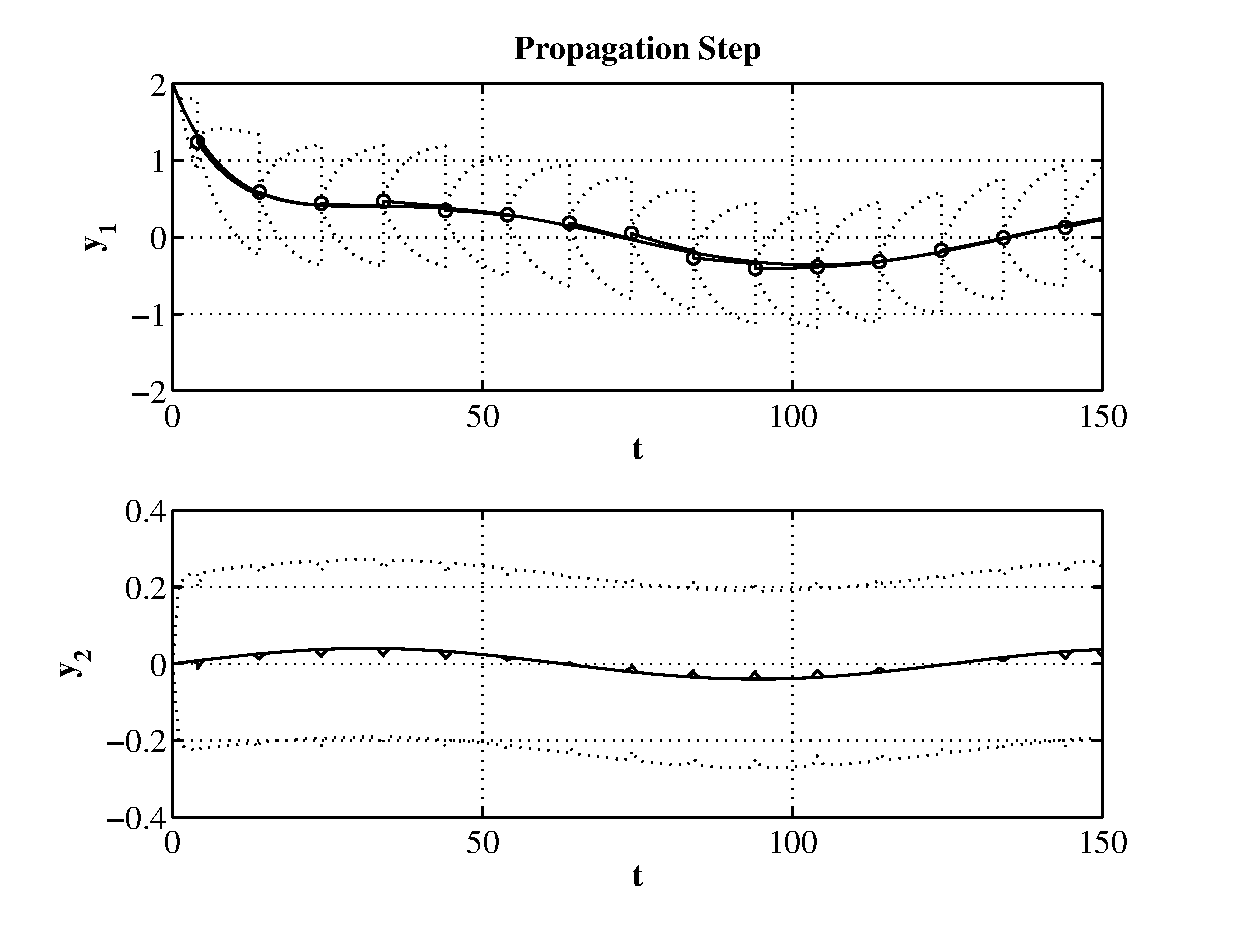
\includegraphics[width=\textwidth]{2g}
        \caption{Kalman filter estimate for 150 time steps}
        \label{2g}
\end{figure}
\end{document}
